\section{\Glsfmtlongpl{rnn}}
\label{sec.rnn}

L'un des principaux défauts que nous avons observés avec les \glspl{mlp} 
et qui nous ont poussés à introduire l'architecture encodeur--décodeur,
est leur incapacité de représenter la dépendance entres les éléments d'une séquence.
Une incapacité qui résulte de leur traitement indépendant des éléments.

Les \glspl{rnn} tentent à résoudre ce problème en utilisant un état interne persistant.
Chaque élément de la séquence modifie cet état lors de son traitement.
Cela permet aux premiers éléments d'affecter le traitement des éléments qui les suivent, 
ainsi permettant à l'information de se propager vers le futur,
ce qui donne lieu à une \emph{mémoire}.
\begin{figure}[hbt]
    \begin{center}
        \begin{subfigure}{.4\linewidth}
            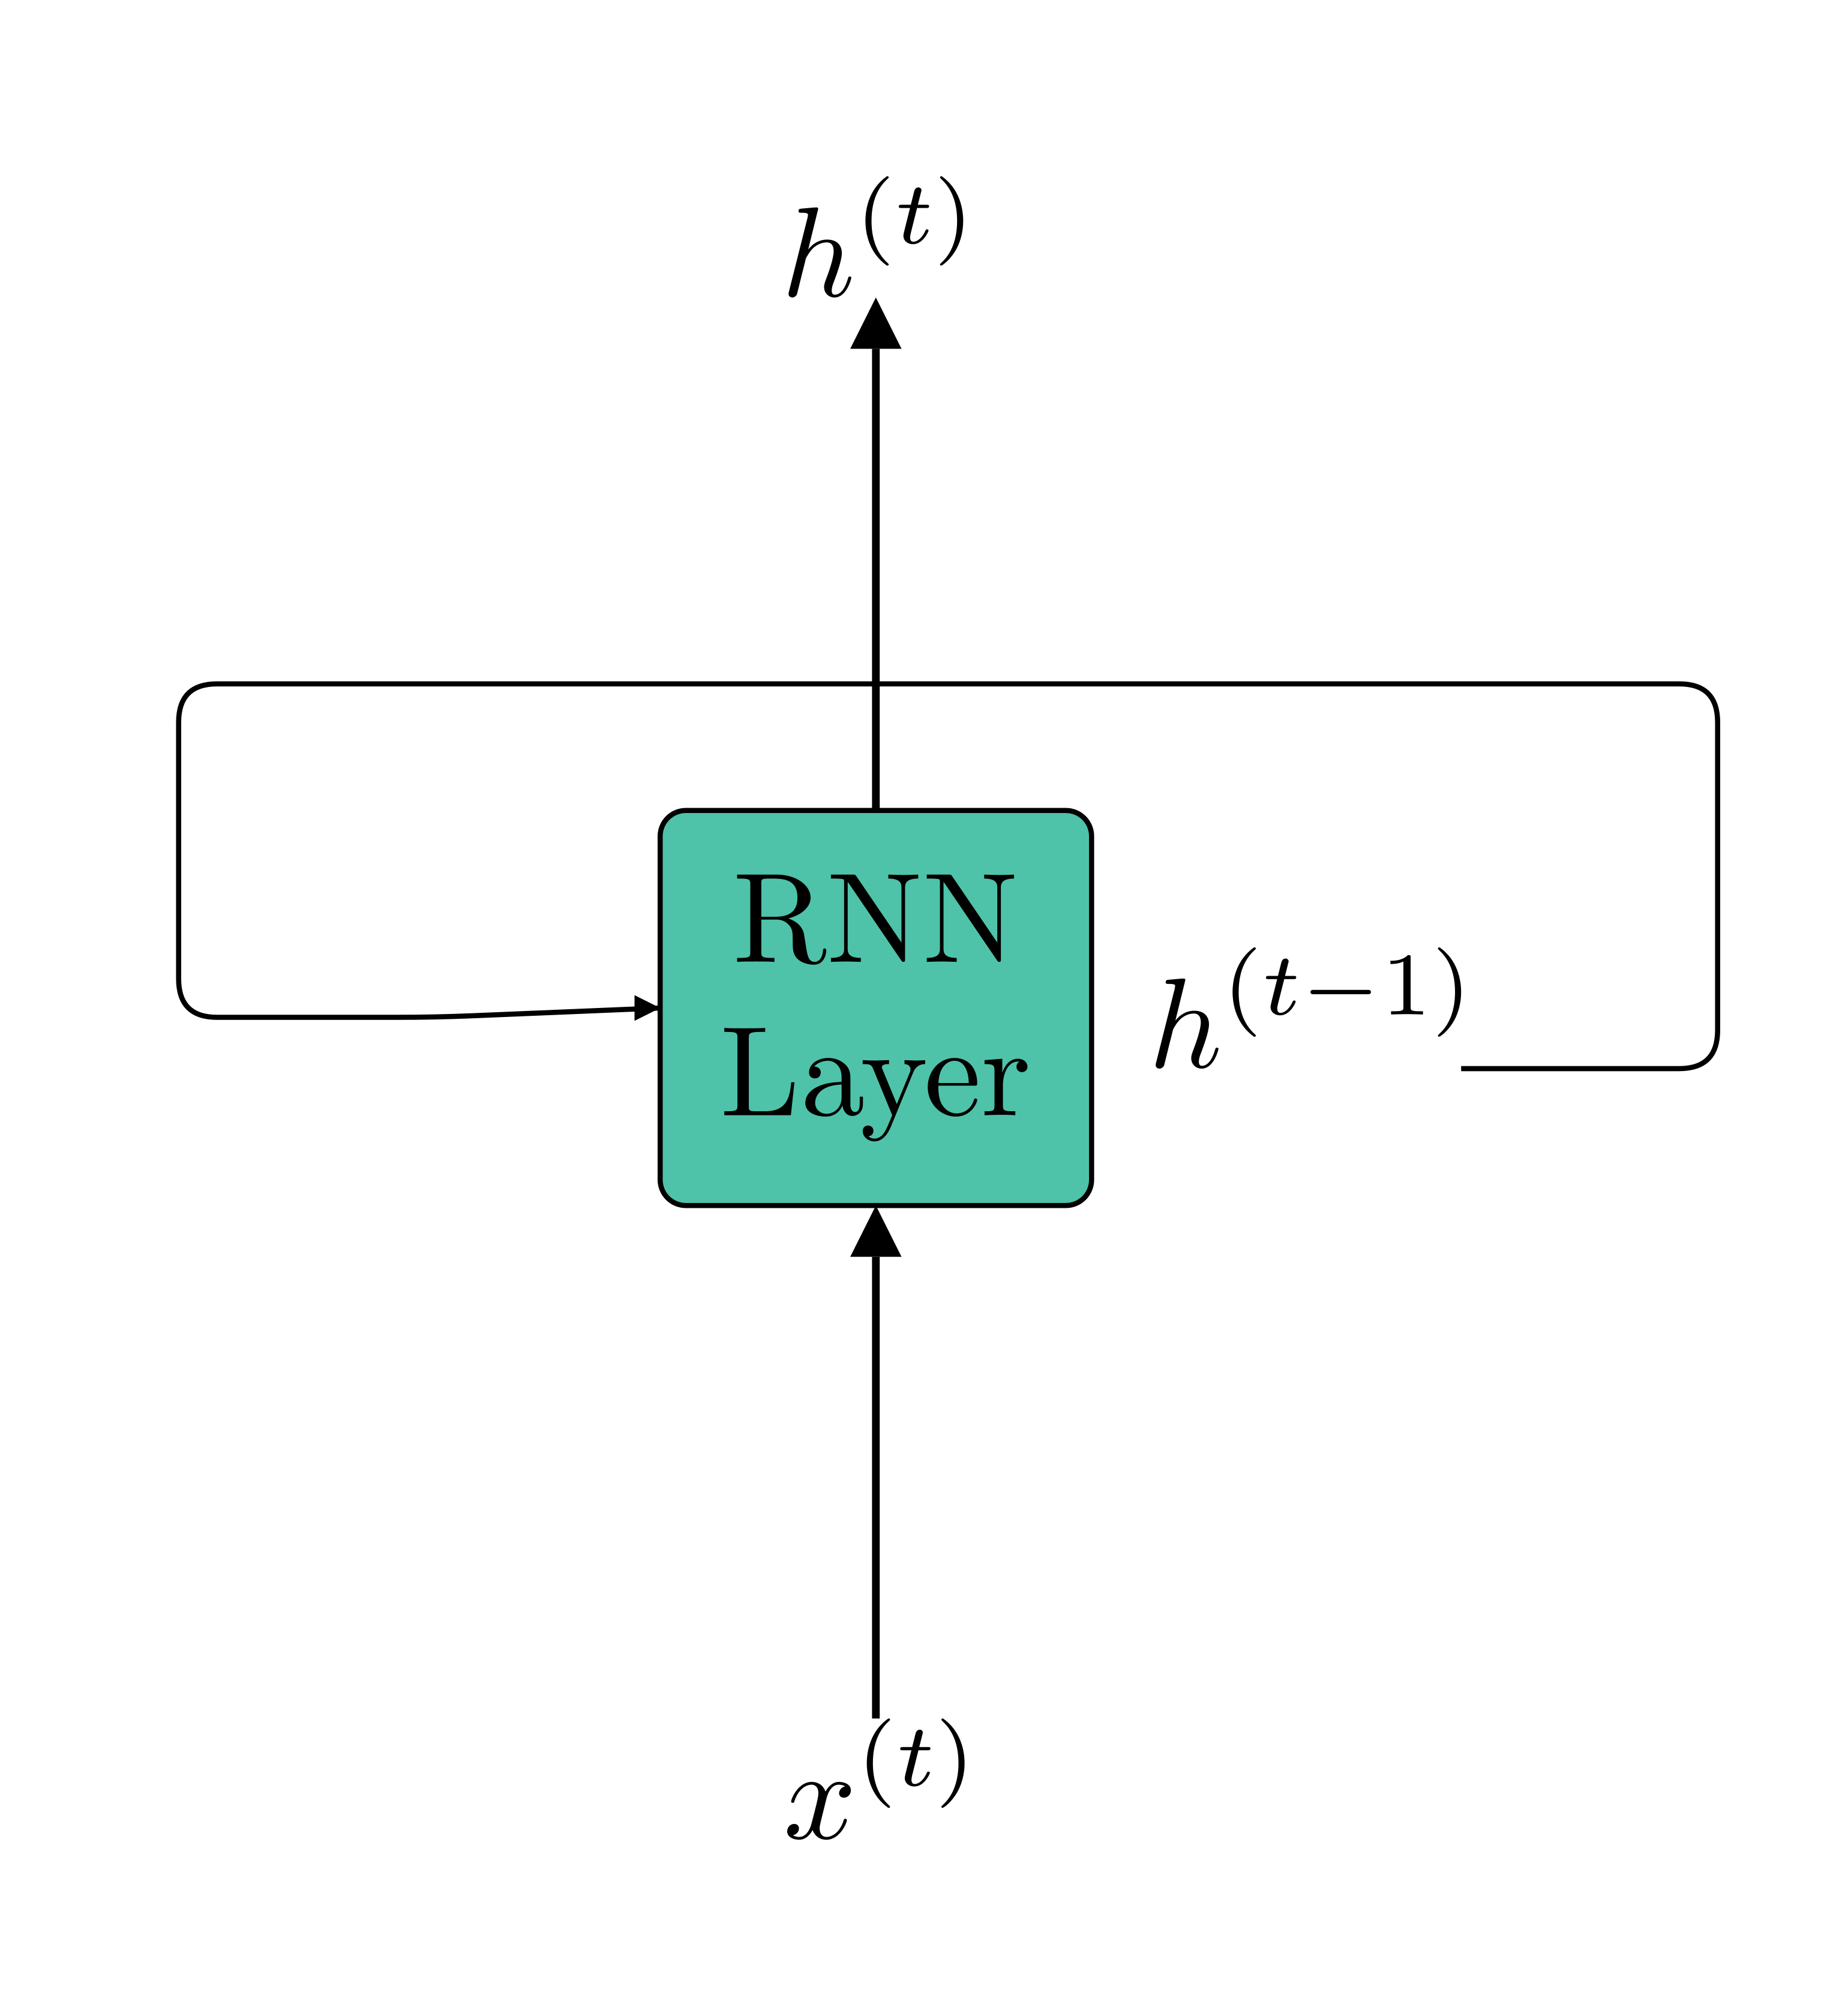
\includegraphics[width=\linewidth]{assets/images/rnn-loop}
            \caption{Couche récurrente}
            \label{fig.rnn-loop}
        \end{subfigure}
        \begin{subfigure}{.4\linewidth}
            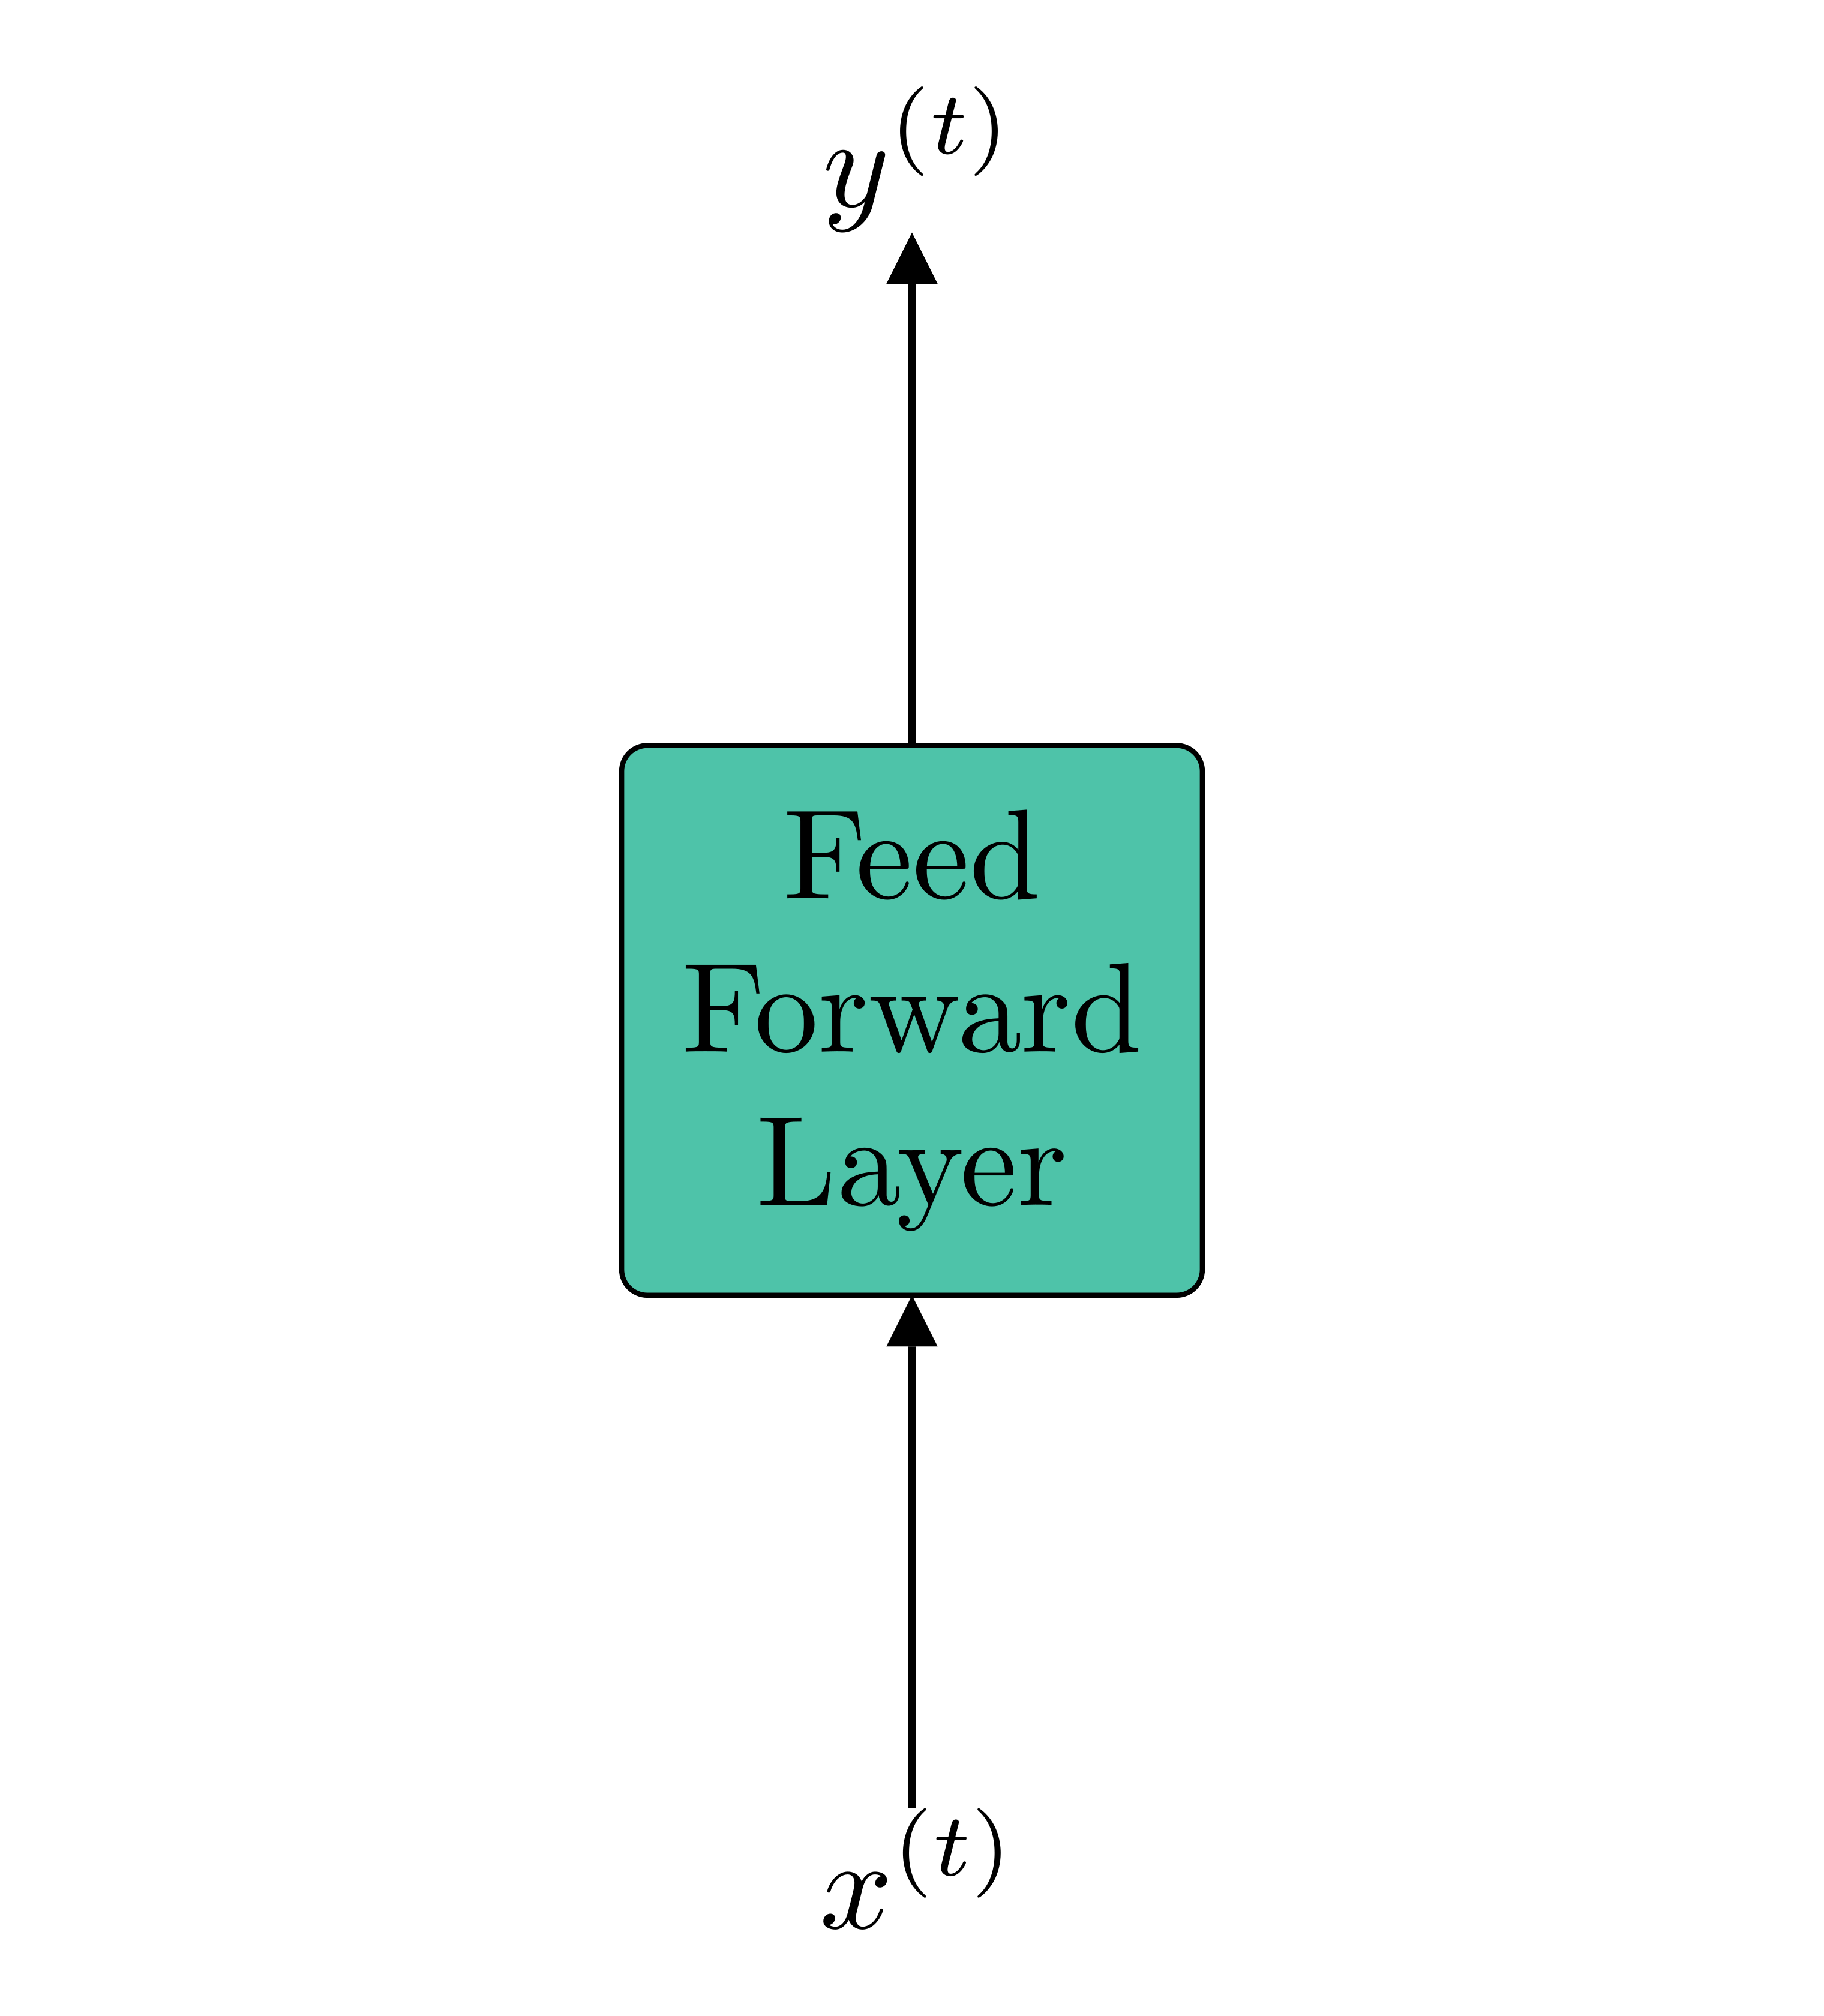
\includegraphics[width=\linewidth]{assets/images/ffn-layers}
            \caption{Couche feed-forward}
            \label{fig.ffn-layer}
        \end{subfigure}
    \end{center}
    \caption{\glsfmtshort{rnn} v.s \glsfmtshort{ffn}}
    \label{fig.rnn-vs-ffn}
\end{figure}
Pour implémenter ce type de comportement, 
l'état d'un \gls{rnn} est décalé d'une unité est réinjecté dans l'entrée (Voire Figure~\ref{fig.rnn-loop}).
Cela est très différent des \glspl{mlp} qui n'ont pas de boucle de rétroaction,
il s'agit de \glspl{ffn} (Voire Figure~\ref{fig.ffn-layer}).
Par conséquent, ils n'ont pas d'état ni de mémoire~\cite{Fathi_2021}.


\subimport{}{simple}
\subimport{}{lstm-gru}
